

This section will talk about Magnetostriction and the physics involved in it. 

Unpaired electrons in the valence shell, or unbalanced spins, can produce significant magnetism in an atom.  However, these electrons are used in bonding when forming a solid making their contribution to magnetism in a solid is negligible\cite{Breu2008}.  The preserved magnetic moments in solids are more characteristic of an element’s ionic electron configuration (Fe{$^{3+}$} rather than Fe) or with sufficient bonding electrons added to complete the shell.  The only groups of elements in the periodic table which exhibit magnetic moments in solids are those in which the unbalanced electron populations occur in an inner shell, namely the transition metals (3\textit{d}, 4\textit{d}, and 5\textit{d}), rare earths (4\textit{f}), and actinides (5\textit{f}).  It is clear that the more tightly bound an unfilled orbital shell is, the less the unpaired electrons will have to do with bonding and the more they will contribute to magnetism.  This is why we see very strong magnetic responses in rare earth materials which use 6\textit{s} and 5\textit{d} shells for bonding before using the very tightly bound 4\textit{f} shell electrons.  The 3\textit{d} electrons in transition metals are less tightly bound to the nucleus, and sometimes 3\textit{d} electrons are used for bonding.  \\

\begin{figure}[h] 
	\centering
	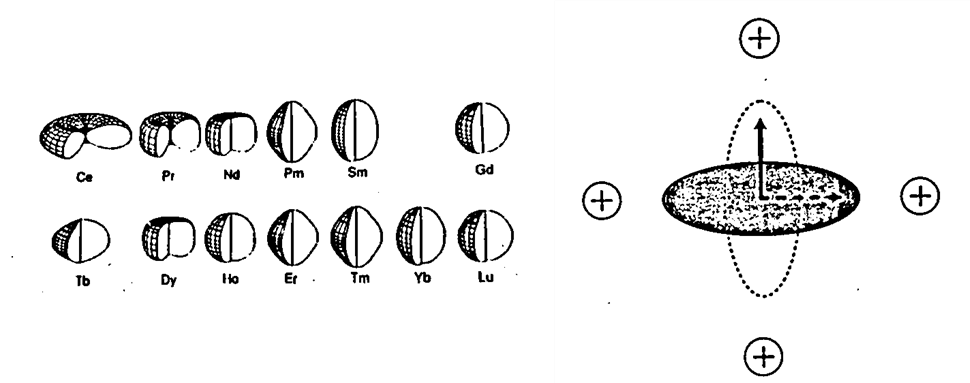
\includegraphics[trim=0pt 10pt 0pt 0pt,scale=1.0]{electron_cloud_density}
	\caption{(a) 4f electron charge cloud densities for a number of rare earth elements. (b) Schematic of oblate 4f charge density of a rare earth element with + nearest neighbors, such as Tb, rotating in a magnetic field. \cite{Engdahl1999} 
	}
	\label{fig:electron_cloud_density}		
\end{figure}

Magneto-elasticity is the coupling between a material’s classical properties of elasticity and strain and the quantum mechanical and relativistic phenomena of magnetism.  When a spin imbalance occurs, electrons can order in such a way that the net magnetic moment points in a particular direction which lowers the crystal symmetry and produces new properties, like magnetostriction.\cite{Breu2008} This coupling between magnetism and elasticity derives from the large contribution of the spin moment to the magnetic moment.  Hence, coupling occurs if there is a strong coupling between the \textit{direction} of the atom’s spin moment and the \textit{orientation} of its anisotropically shaped electron charge cloud, as seen in Figure 1a.  This coupling that exists at the individual electron level is called “spin-orbit coupling,” and since it derives from relativistic aspects of the electron motion, it is one of the smallest energies used to describe the state of an atom.  It is easiest to see this coupling in rare earth elements where the spin directions of rapidly moving 4\textit{f} electrons are strongly coupled to the orientation of their orbits.  This individual electron spin-orbit coupling leads to strong coupling between the total spin moment and the total electron density.  Thus, in rare earth elements the spin moment can be envisioned as rigidly attached to the anisotropically shaped electron charge cloud.  We can now define magnetic anisotropy as the tendency of a magnetic moment to point in a specific crystalline direction, the easy magnetization direction, because of the electrical attraction/repulsion between the rotating electronic charge cloud and neighboring charged ions, as seen in Figure 1b.  It is important to note that 3d electrons obey the same magnetoelastic trends, but with a factor of ten less for spin-orbit coupling.\cite{Engdahl1999}
